\tikzstyle{input_neuron}=[circle,draw=red!50,fill=orange!10,thick,minimum size=.2mm]
\tikzstyle{hidden_neuron}=[circle,draw=blue!50,fill=blue!10,thick,minimum size=1mm]
\tikzstyle{output_neuron}=[circle,draw=green!50,fill=green!20,thick,minimum size=1mm]
\tikzstyle{input}=[circle,draw=black!50,fill=black!20,thick,minimum size=.2mm]
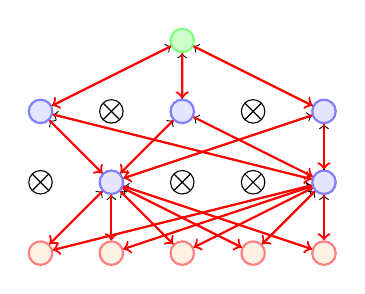
\begin{tikzpicture}[scale=.9, transform shape,cross/.style={path picture={ 
		\draw[black]
		(path picture bounding box.south east) -- (path picture bounding box.north west) (path picture bounding box.south west) -- (path picture bounding box.north east);
	}}]]
	\tikzstyle{mynode} = [draw,shape=circle]
	\tikzstyle{mycross} = [draw,shape=circle,cross]
	\node[input_neuron,mynode] (a0) at (0, 0) {};
	\node[input_neuron,mynode] (a1) at (1, 0) {};
	\node[input_neuron,mynode] (a2) at (2, 0) {};
	\node[input_neuron,mynode] (a3) at (3, 0) {};
	\node[input_neuron,mynode] (a4) at (4, 0) {};
	\node[mycross] (b0) at (0, 1) {};
	\node[hidden_neuron,mynode] (b1) at (1, 1) {};
	\node[mycross] (b2) at (2, 1) {};
	\node[mycross] (b3) at (3, 1) {};
	\node[hidden_neuron,mynode] (b4) at (4, 1) {};
	\node[hidden_neuron,mynode] (c0) at (0, 2) {};
	\node[mycross] (c1) at (1, 2) {};
	\node[hidden_neuron,mynode] (c2) at (2, 2) {};
	\node[mycross] (c3) at (3, 2) {};
	\node[hidden_neuron,mynode] (c4) at (4, 2) {};
	\node[output_neuron,mynode] (d2) at (2, 3) {};
	\foreach \from in {a0,a1,a2,a3,a4}
		\foreach \to in {b1,b4}
			\draw [->] (\from) -- (\to);
	\foreach \from in {b1,b4}
		\foreach \to in {c0,c2,c4}
			\draw [->] (\from) -- (\to);
	\foreach \from in {c0,c2,c4}
		\draw [->] (\from) -- (d2);
	\foreach \from in {c0,c2,c4}
		\draw<1-> [thick,red,->] (d2) -- (\from);
	\foreach \from in {b1,b4}
		\foreach \to in {c0,c2,c4}
			\draw<1-> [thick,red,->] (\to) -- (\from);
	\foreach \from in {a0,a1,a2,a3,a4}
		\foreach \to in {b1,b4}
			\draw<1-> [thick,red,->] (\to) -- (\from);
\end{tikzpicture}